%----------------------------------------------------------------------------------------
%   PACKAGES AND OTHER DOCUMENT CONFIGURATIONS
%----------------------------------------------------------------------------------------

\documentclass[a4paper, 12pt]{article} % A4 paper and 11pt font size

\usepackage[T1]{fontenc} % Use 8-bit encoding that has 256 glyphs
\usepackage{fourier} % Use the Adobe Utopia font for the document - comment this line to return to the LaTeX default
\usepackage[english]{babel} % English language/hyphenation
\usepackage{amsmath,amsfonts,amsthm} % Math packages

\usepackage{sectsty} % Allows customizing section commands
\allsectionsfont{\raggedright \normalfont\scshape} % Make all sections centered, the default font and small caps

\usepackage{fancyhdr} % Custom headers and footers
\pagestyle{fancyplain} % Makes all pages in the document conform to the custom headers and footers
\fancyhead{} % No page header - if you want one, create it in the same way as the footers below
\fancyfoot[L]{} % Empty left footer
\fancyfoot[C]{} % Empty center footer
\fancyfoot[R]{\thepage} % Page numbering for right footer
\renewcommand{\headrulewidth}{0pt} % Remove header underlines
\renewcommand{\footrulewidth}{0pt} % Remove footer underlines
\setlength{\headheight}{13.6pt} % Customize the height of the header

\usepackage{parskip}
\setlength{\parindent}{15pt}
 \usepackage{graphicx}
 \usepackage{epstopdf}
\usepackage{caption}
\usepackage{subcaption}
%\numberwithin{equation}{section} % Number equations within sections (i.e. 1.1, 1.2, 2.1, 2.2 instead of 1, 2, 3, 4)
%\numberwithin{figure}{section} % Number figures within sections (i.e. 1.1, 1.2, 2.1, 2.2 instead of 1, 2, 3, 4)
%\numberwithin{table}{section} % Number tables within sections (i.e. 1.1, 1.2, 2.1, 2.2 instead of 1, 2, 3, 4)

\setlength\parindent{0pt} % Removes all indentation from paragraphs - comment this line for an assignment with lots of text

%----------------------------------------------------------------------------------------
%   TITLE SECTION
%----------------------------------------------------------------------------------------

\newcommand{\horrule}[1]{\rule{\linewidth}{#1}} % Create horizontal rule command with 1 argument of height

\title{ 
\normalfont \normalsize 
\textsc{Nuclear Engineering, UC Berkeley} \\ [25pt] % Your university, school and/or department name(s)
\horrule{0.5pt} \\[0.4cm] % Thin top horizontal rule
\huge NE 255 HOMEWORK 3: Monte Carlo Modeling with Serpent \\  % The assignment title
\horrule{2pt} \\[0.5cm] % Thick bottom horizontal rule
}

\author{Xin Wang} % Your name

\date{\normalsize\today} % Today's date or a custom date


\begin{document}

%----------------------------------------------------------------------------------------
%   Problem 2.c
%----------------------------------------------------------------------------------------
\section*{Problem 2.c}

a)

$k_{eff} = 1.51595E+00 \pm 0.00184$

b)

The average neutron flux in the fuel is $1.46362E+1 \pm 0.00177$, in the clad is $4.71467 \pm 0.00221$, in the moderator is $2.39584E01 \pm 0.00144$.

c)

The average absorption rate is $3.82027 \pm 0.00746$ and the average fission rates in the fuel is $41.89417 \pm 0.00172$

d)

The neutron spectrum in 23 energy groups in fuel and modrator is plotted as in figure 1. The neutron population is dominately in the thermal region. It drops rapidely in high energy region. From the two energy group results, we observe that the fast neutron flux is only 1/10 of the thermal neutron flux.  

\begin{figure}
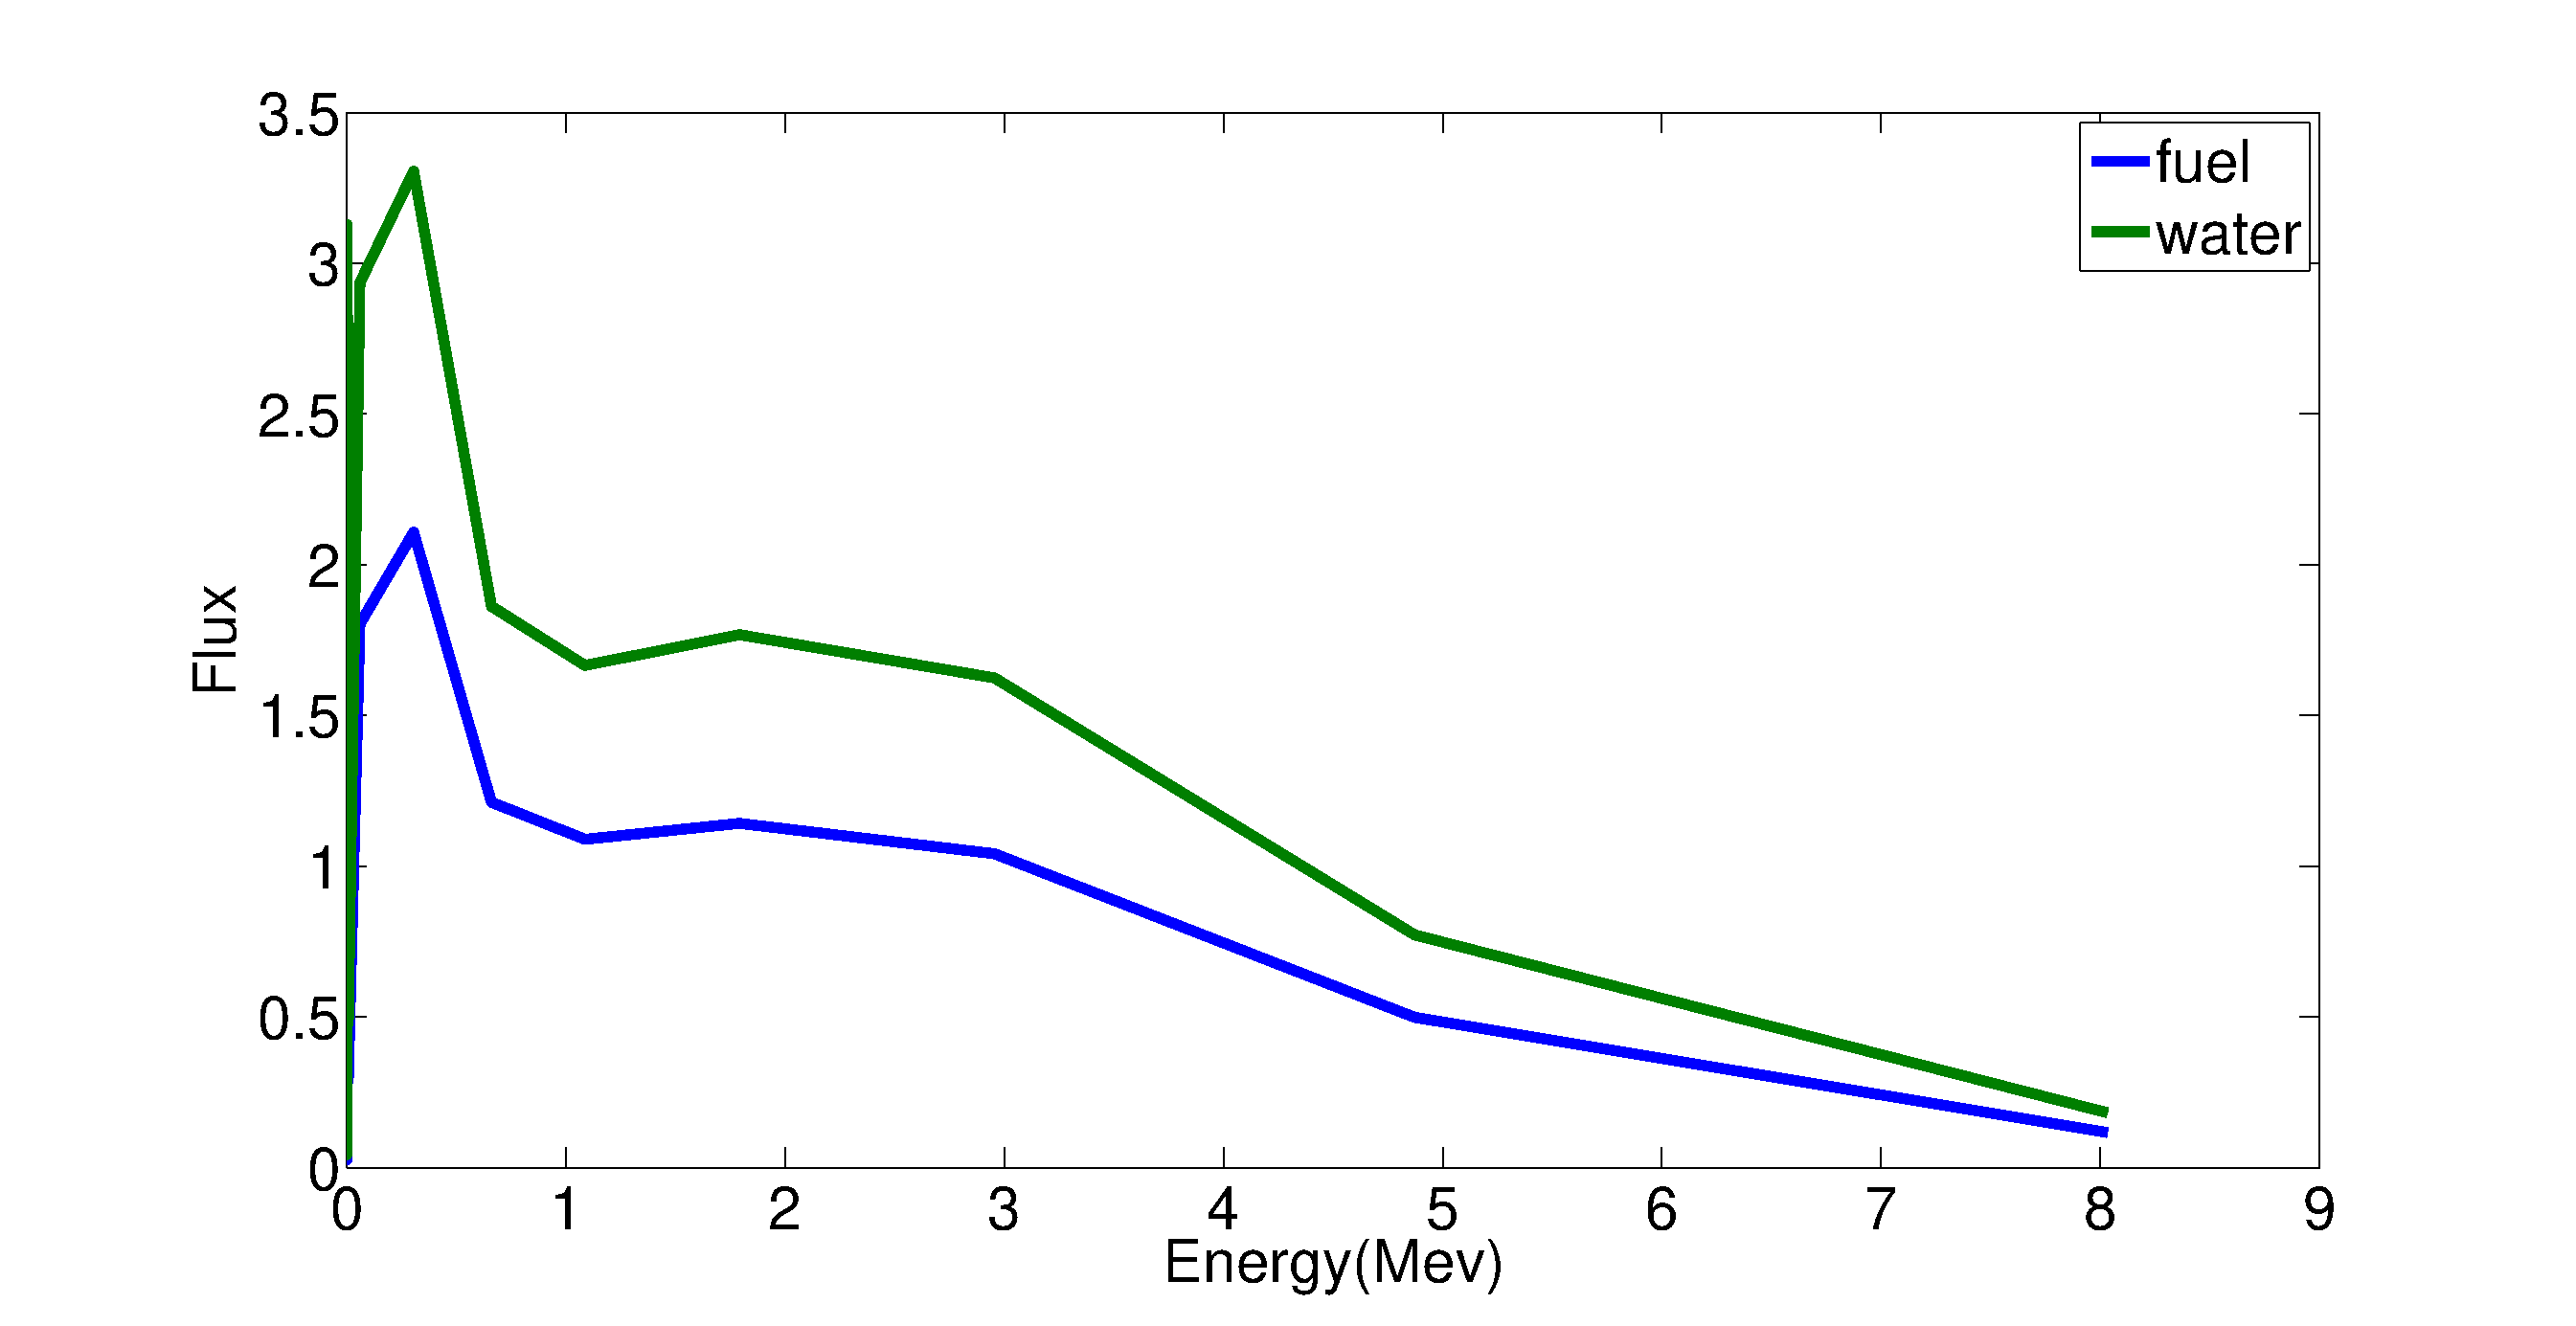
\includegraphics[width = \textwidth]{energy_23_fuel.eps}

\caption{Neutron energy spectrum in fuel and in water}
\label{neutron_spectrum_u02}
\end{figure}

The two group flux in fuel is 
\begin{eqnarray}
\phi_1 = 1.40452 \pm 0.00196 \nonumber\\
\phi_2 = 13.1956 \pm 0.00173 \nonumber
\end{eqnarray}


The two group flux in water is 
\begin{eqnarray}
\phi_1 = 2.69865 \pm 0.00252 \nonumber\\
\phi_2 = 21.2514 \pm 0.00163 \nonumber
\end{eqnarray}

e)

Spacial distribution of a two-group flux along the central line of the fuel pin is
plotted in figure 2 and in figure 3. Additional sparial subdivision is needed for the code to output the averaged flux in each mesh volume instead of averaging the flux in the whole fuel cell volume.


The flux peaks at the center where the neutron leakage is limited.
\begin{figure}
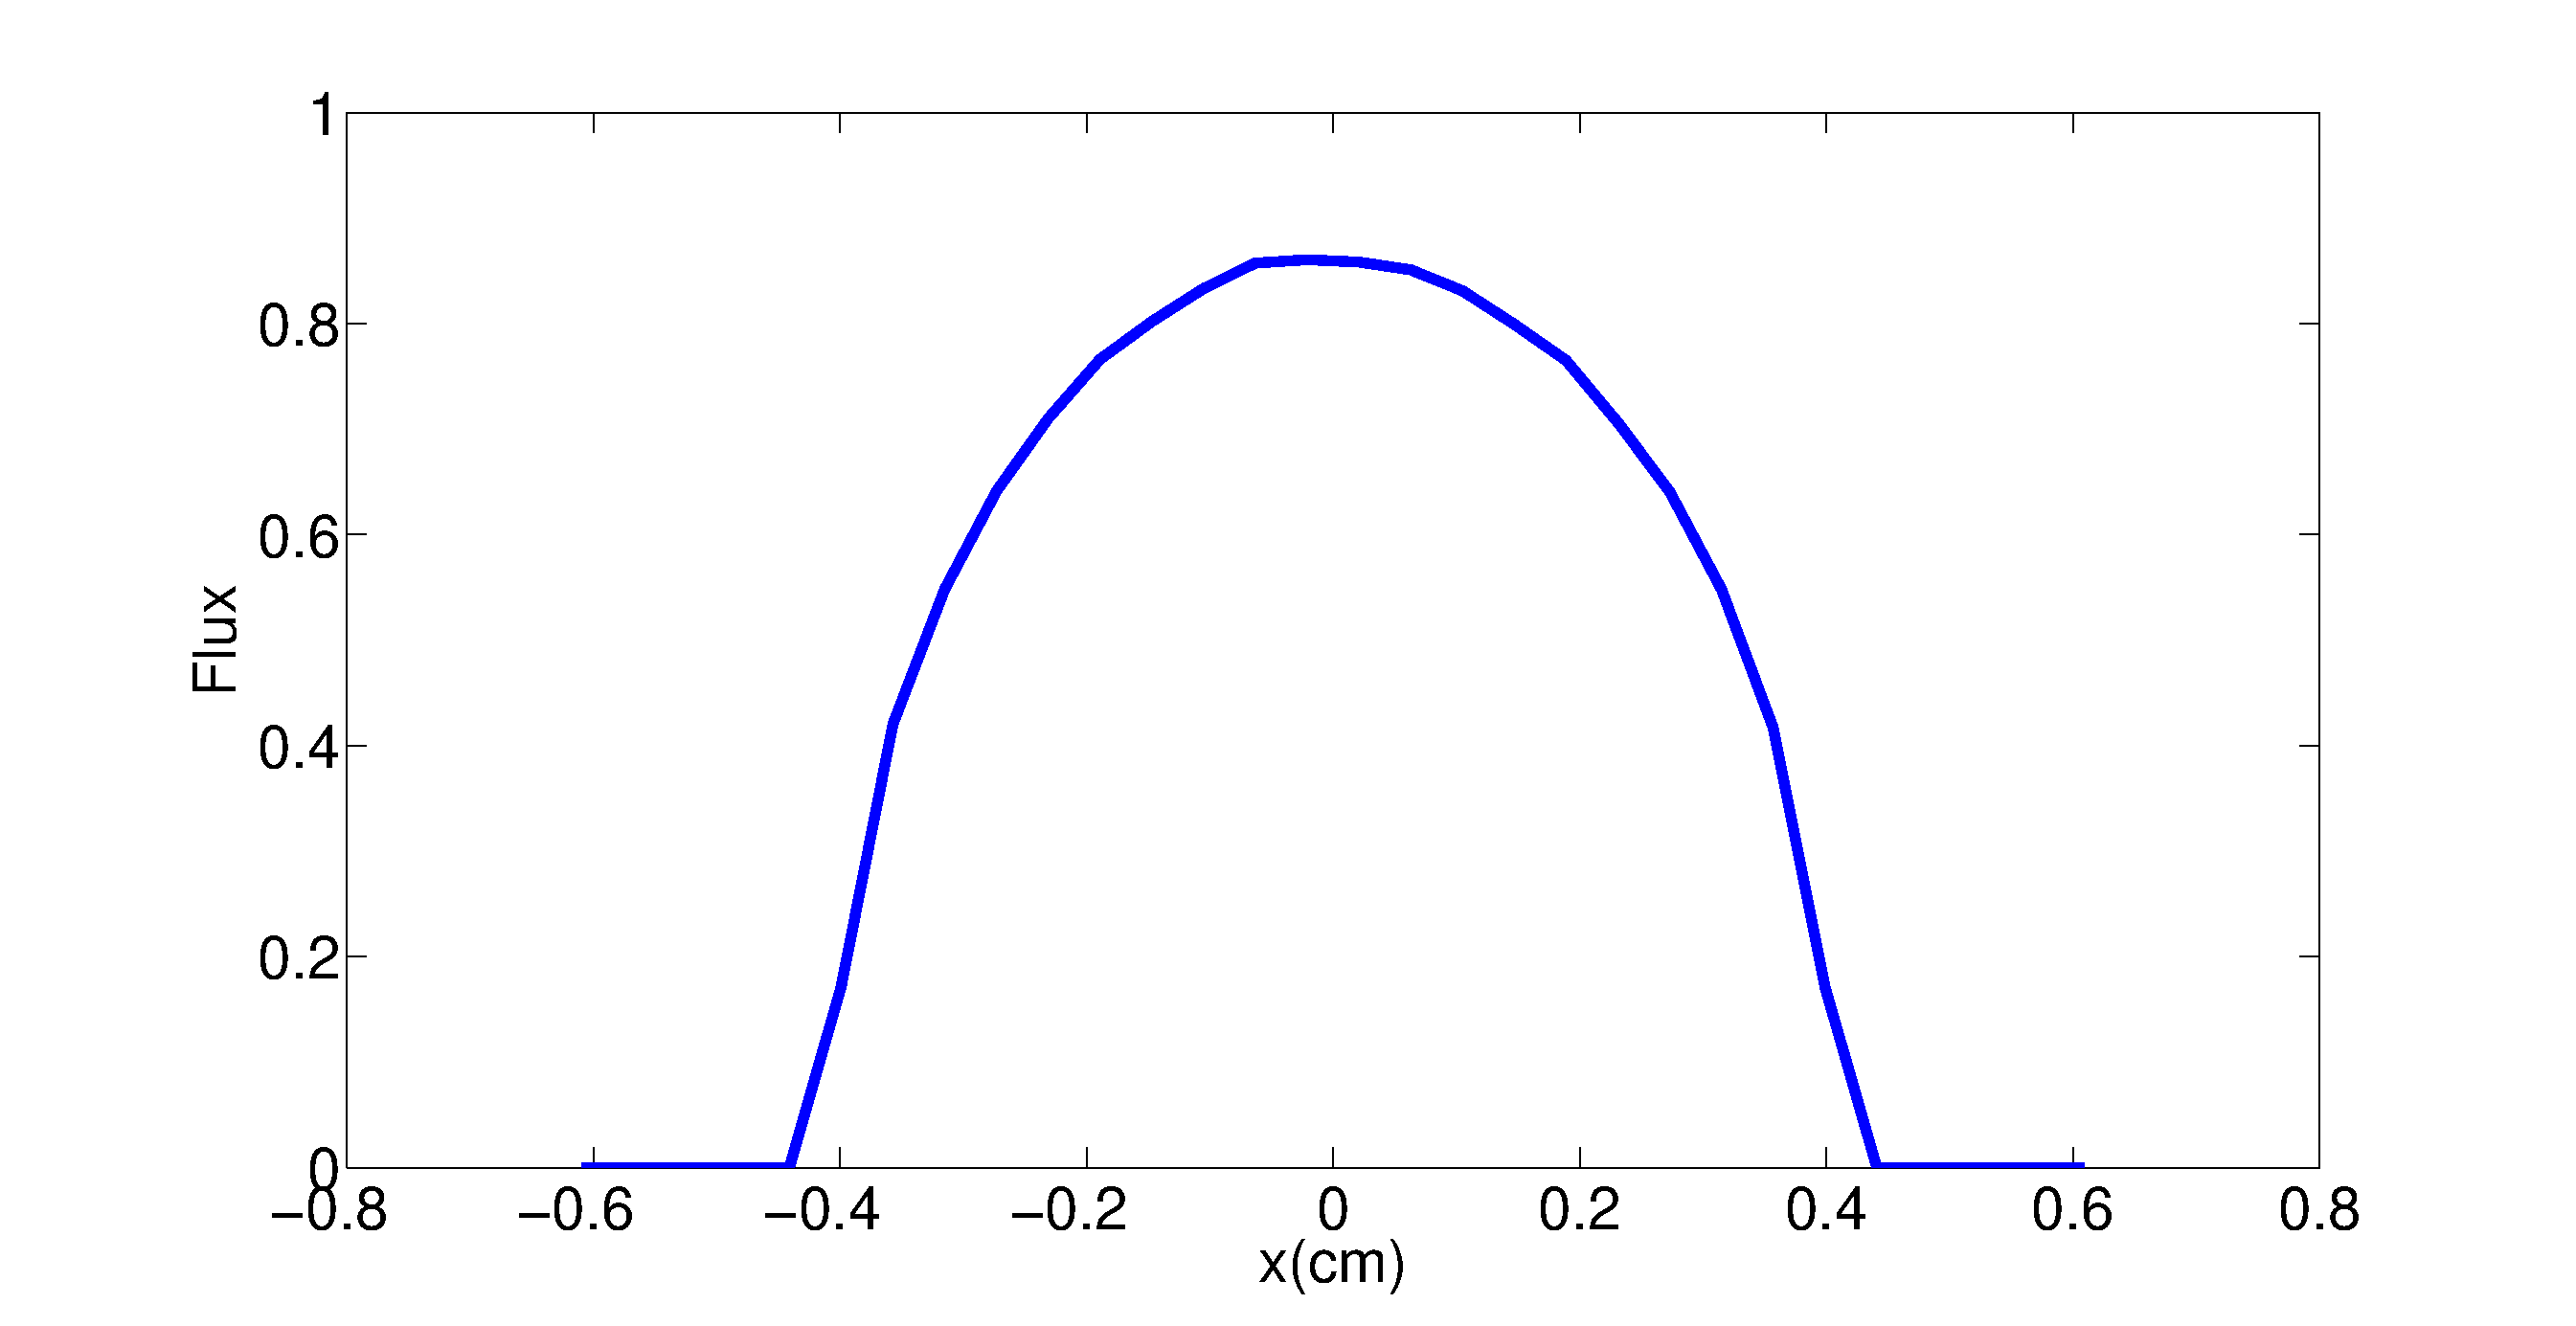
\includegraphics[width = \textwidth]{prob2_x_g1.eps}
\caption{Energy group I neutron flux distribution in fuel}
\end{figure}

\begin{figure}
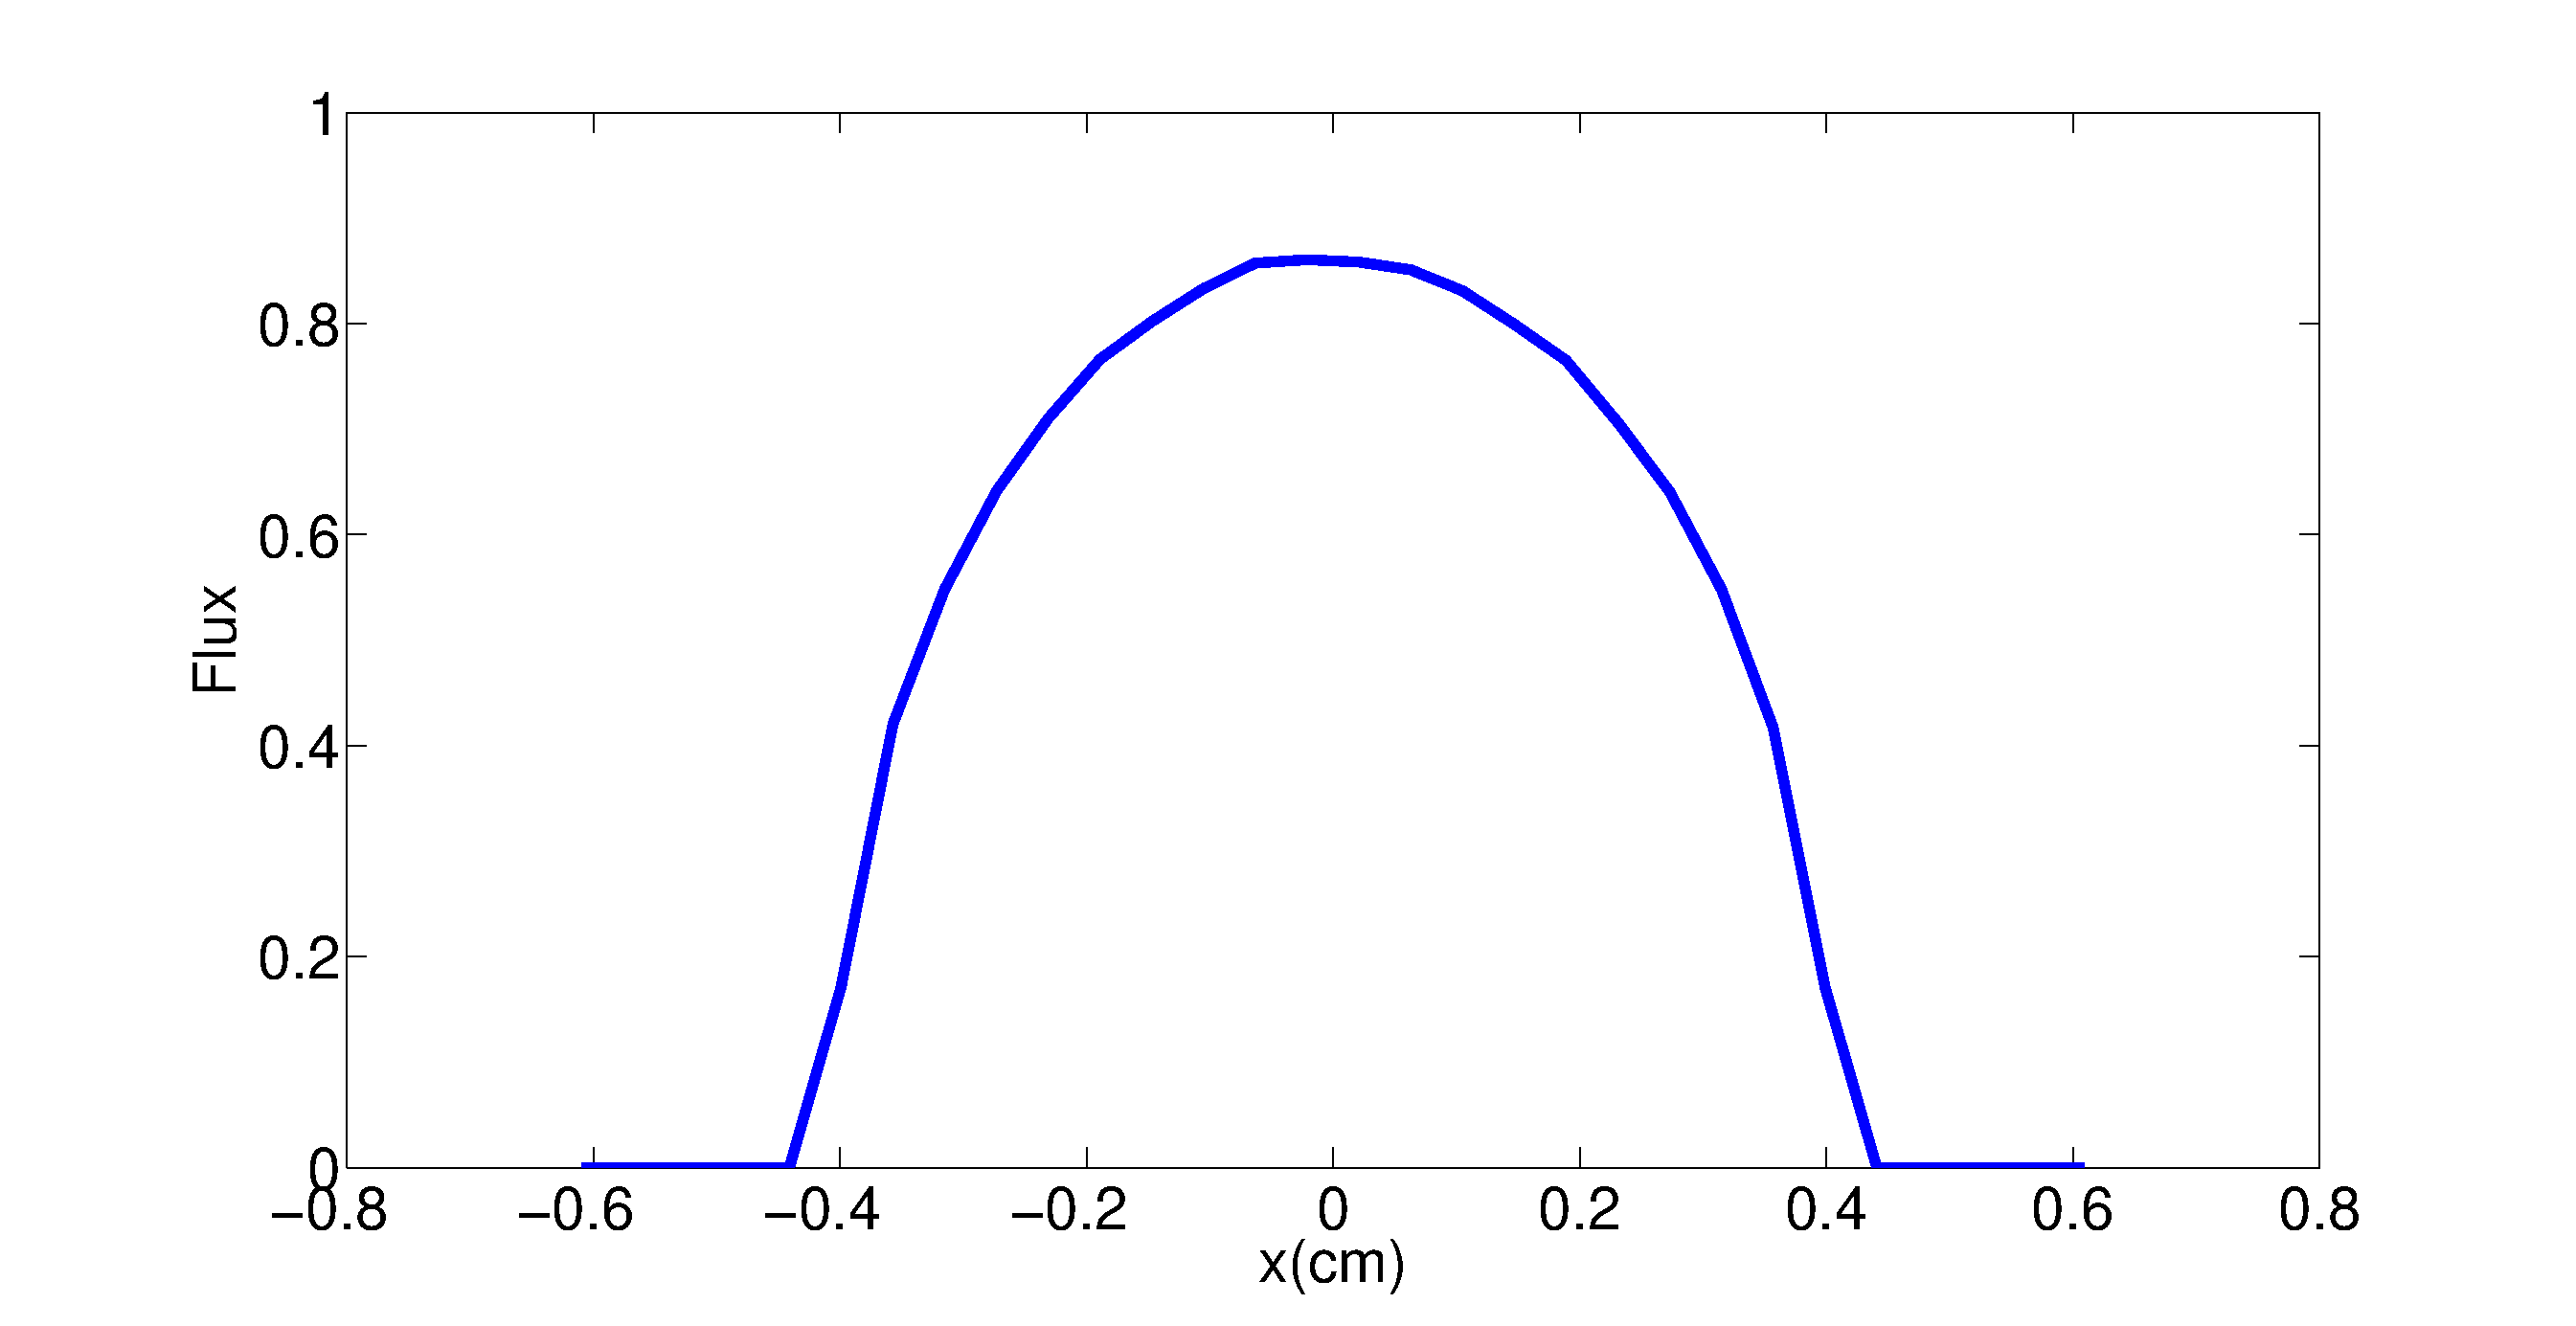
\includegraphics[width = \textwidth]{prob2_x_g2.eps}
\caption{Energy group I neutron flux distribution in fuel}
\end{figure}


%----------------------------------------------------------------------------------------
%   Problem 3
%----------------------------------------------------------------------------------------
\section*{Problem 3}
Defining a lattice constituent with 17 x 17 fuel pins with a pitch of 1.26 cm.

$k_{inf} (analog)= 1.40305 \pm 0.00072$ 
$k_{inf} (implicit)= 1.40279 \pm 0.00036$ 

The difference of $k_{inf}$ between a single pin and a 17x17 fuel pin assembly is not significant, because a single pin with reflective boundary condition is an infinite pin lattice. 

%----------------------------------------------------------------------------------------
%   Problem 4
%----------------------------------------------------------------------------------------
\section*{Problem 4}
The result $k_{inf}$ for different moderator-to-fuel ratio is listed in table and plotted in figure \ref{kinf}

\begin{tabular}{c c c}
pitch & mod-fuel-ratio & $k_{inf}$ \\
1.1   & 0.67 & 1.24610 +/- 0.00135 \\ 
1.26  & 1.19 & 1.37914 +/- 0.00130 \\
1.4   & 1.71 & 1.44844 +/- 0.00120\\
1.6   & 2.53 & 1.49431 +/- 0.00110\\
1.8   & 3.47 & 1.50903 +/- 0.00094 \\
2     & 4.53 & 1.51017 +/- 0.00094
\end{tabular}

\begin{figure}
\caption{kinf vs moderator to fuel ratio}
\label{kinf}
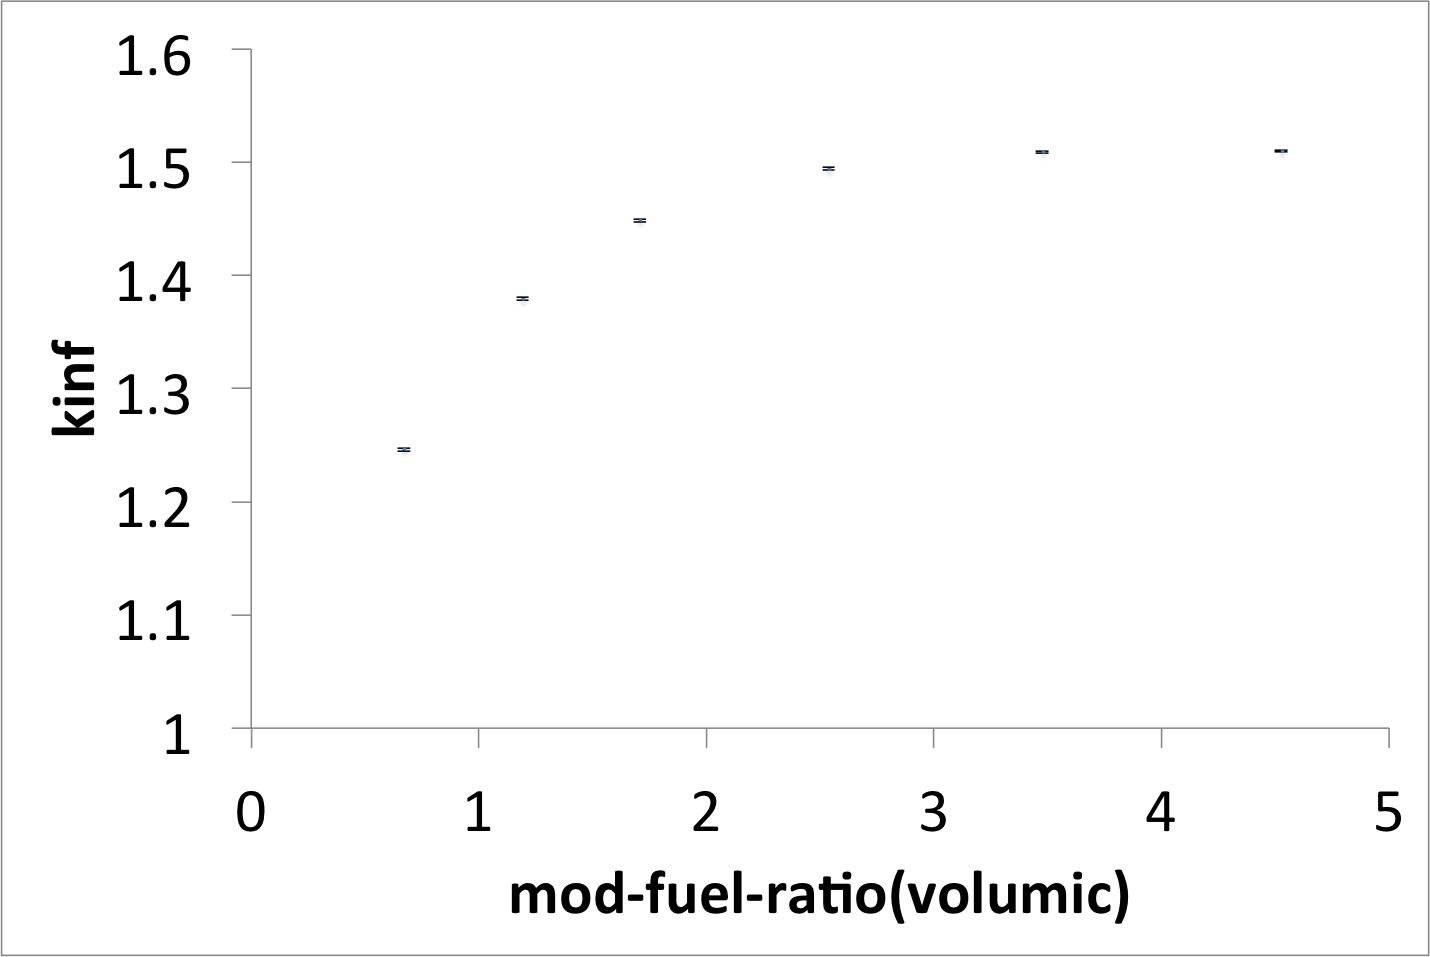
\includegraphics[width = 0.8\textwidth]{kinf_ratio.png}
\end{figure}
%----------------------------------------------------------------------------------------
%   Problem 5
%----------------------------------------------------------------------------------------
\section*{Problem 5}

a)

$k_{eff} = 0.99878 \pm 0.00190$

b)

The average neutron flux in the plutonium sphere is $4.69273\pm0.00195$.

c)

The average absorption rate is $1.06306E-2 \pm 0.00540$. And the average fission rates in the plutonium sphere is $3.17105E-1 \pm 0.00189$

d)

The neutron spectrum is plotted in figure \ref{energy_spec}. The energy spectrum in the Jezabel reactor is faster than the PWR energy spectrum. 

\begin{figure}
\caption{energy spectrum}
\label{energy_spec}
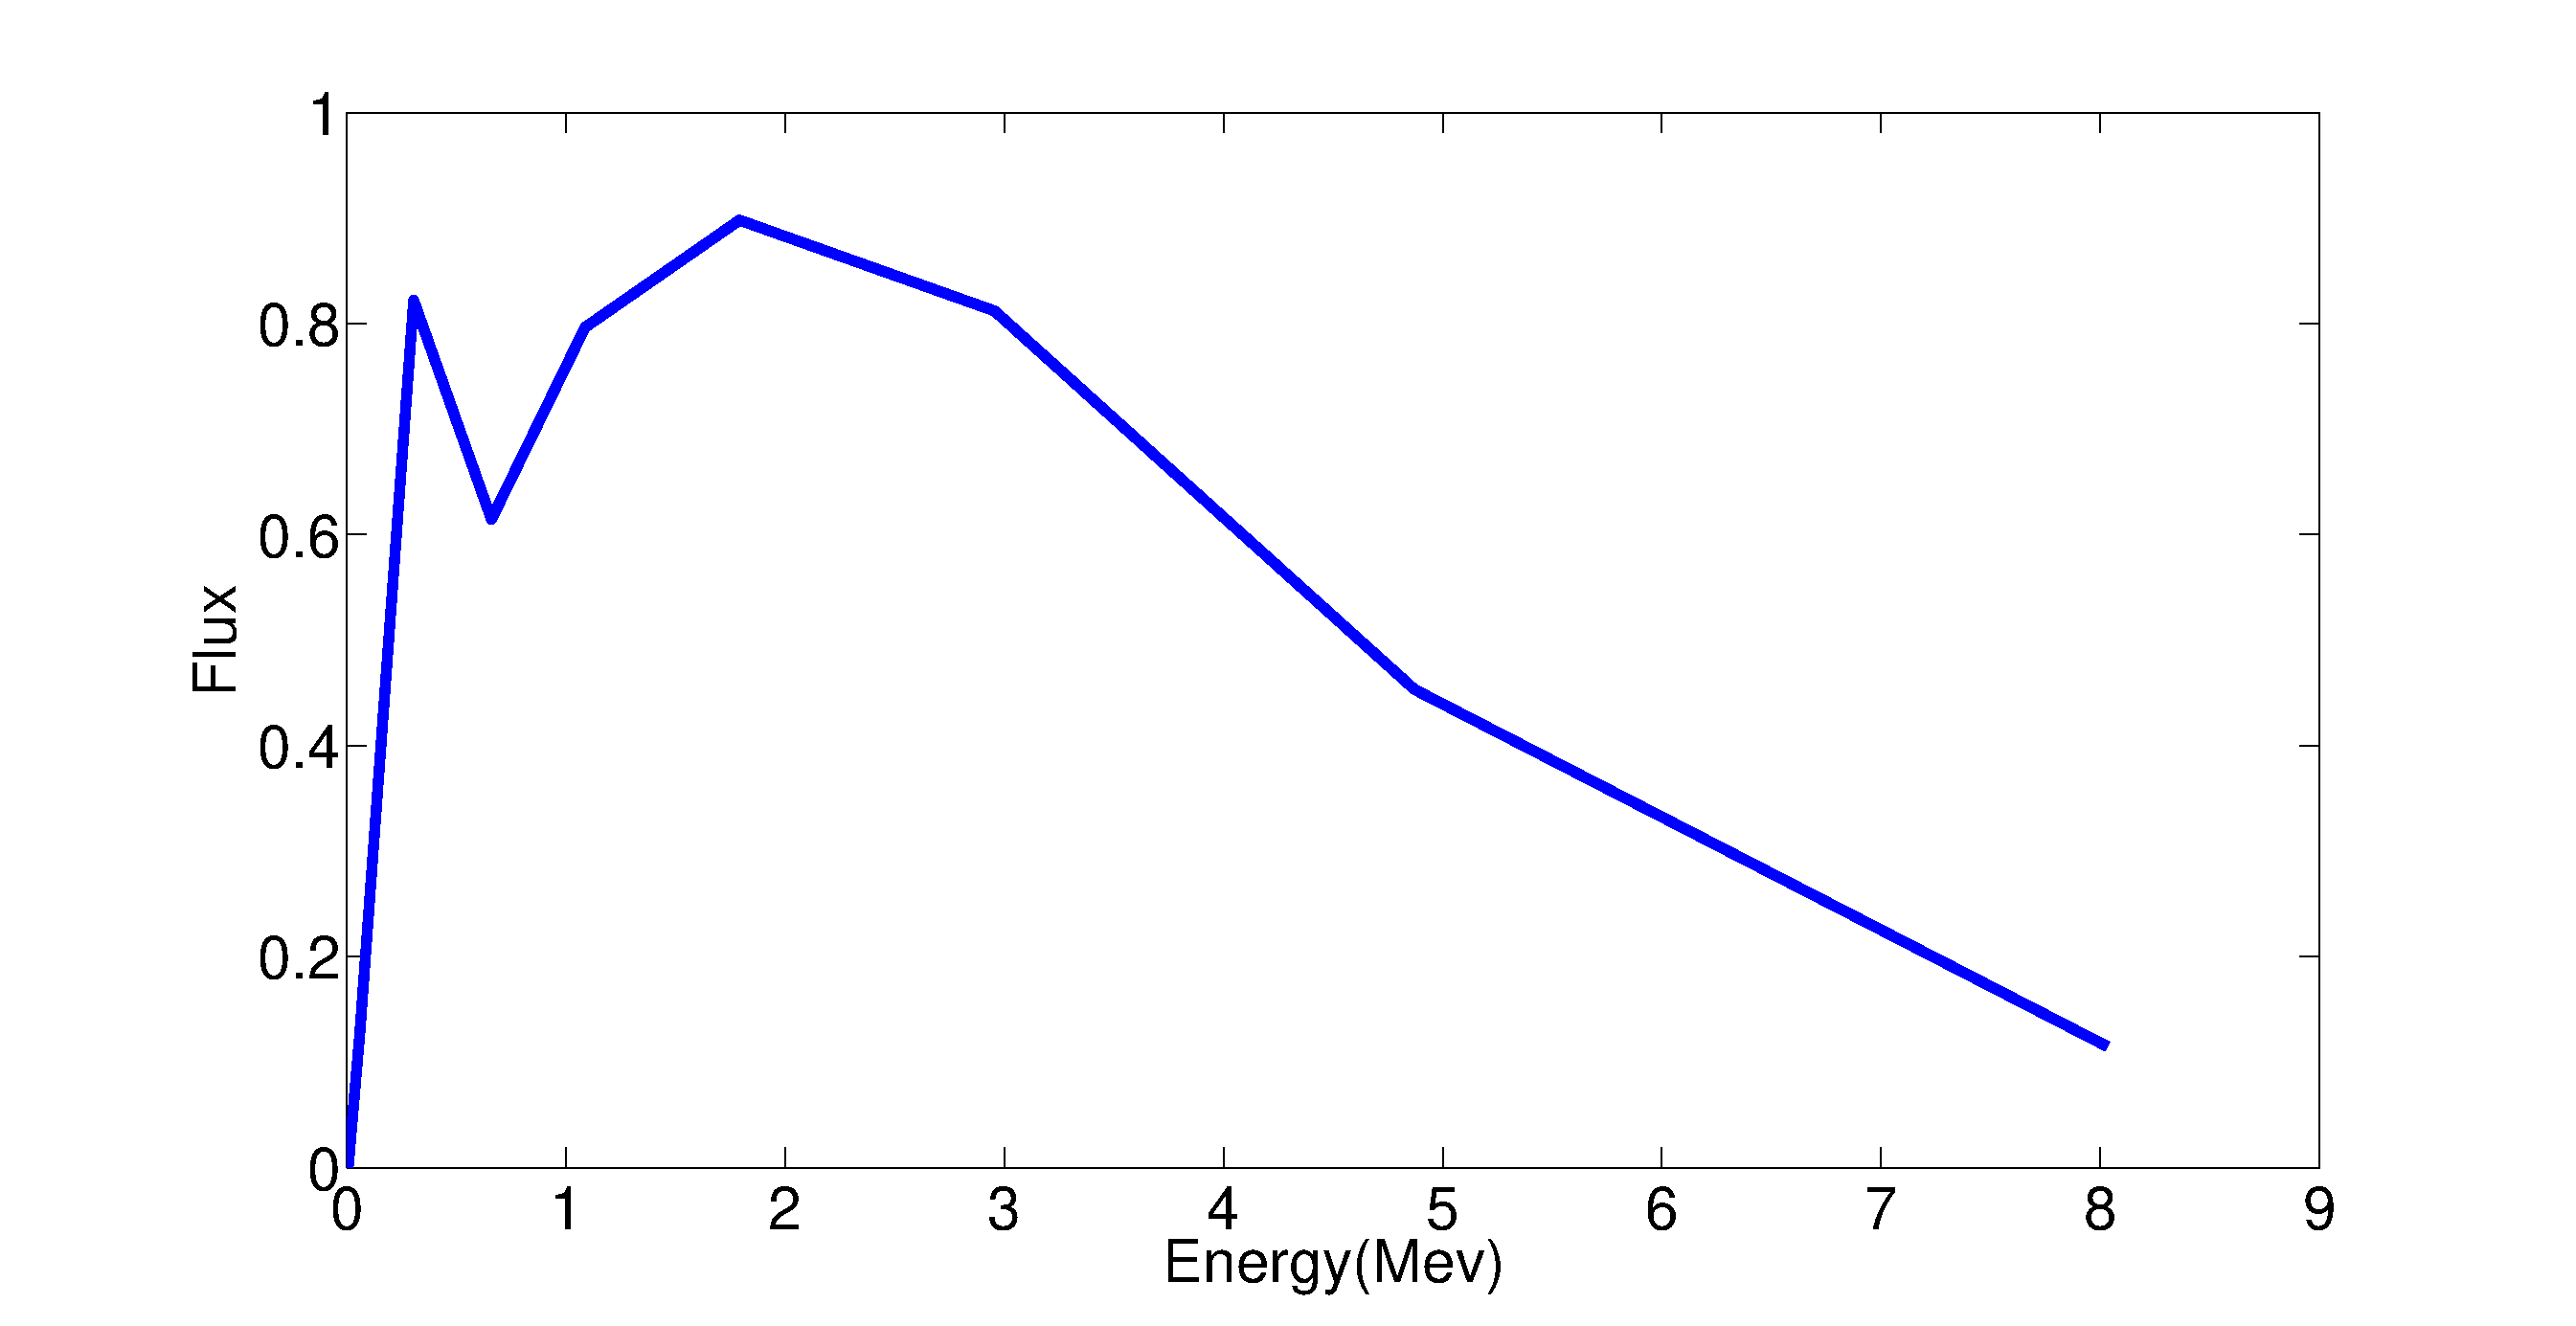
\includegraphics[width = \textwidth]{prob5_energy.eps}
\end{figure}



Two groups spectrum is
$0+0$ for group 1 and 
$4.64096E+00 0.00218$ for group 2

e)

The flux distribution along the central line of the sphere is plotted in figure \ref{flux_x}. Only energy group 2 flux is plotted because group 1 flux is 0.

The distribution is very flat. 
\begin{figure}
\label{flux_x}
\caption{Neutron flux distribution along the central line of the sphere(Energy group 1)}
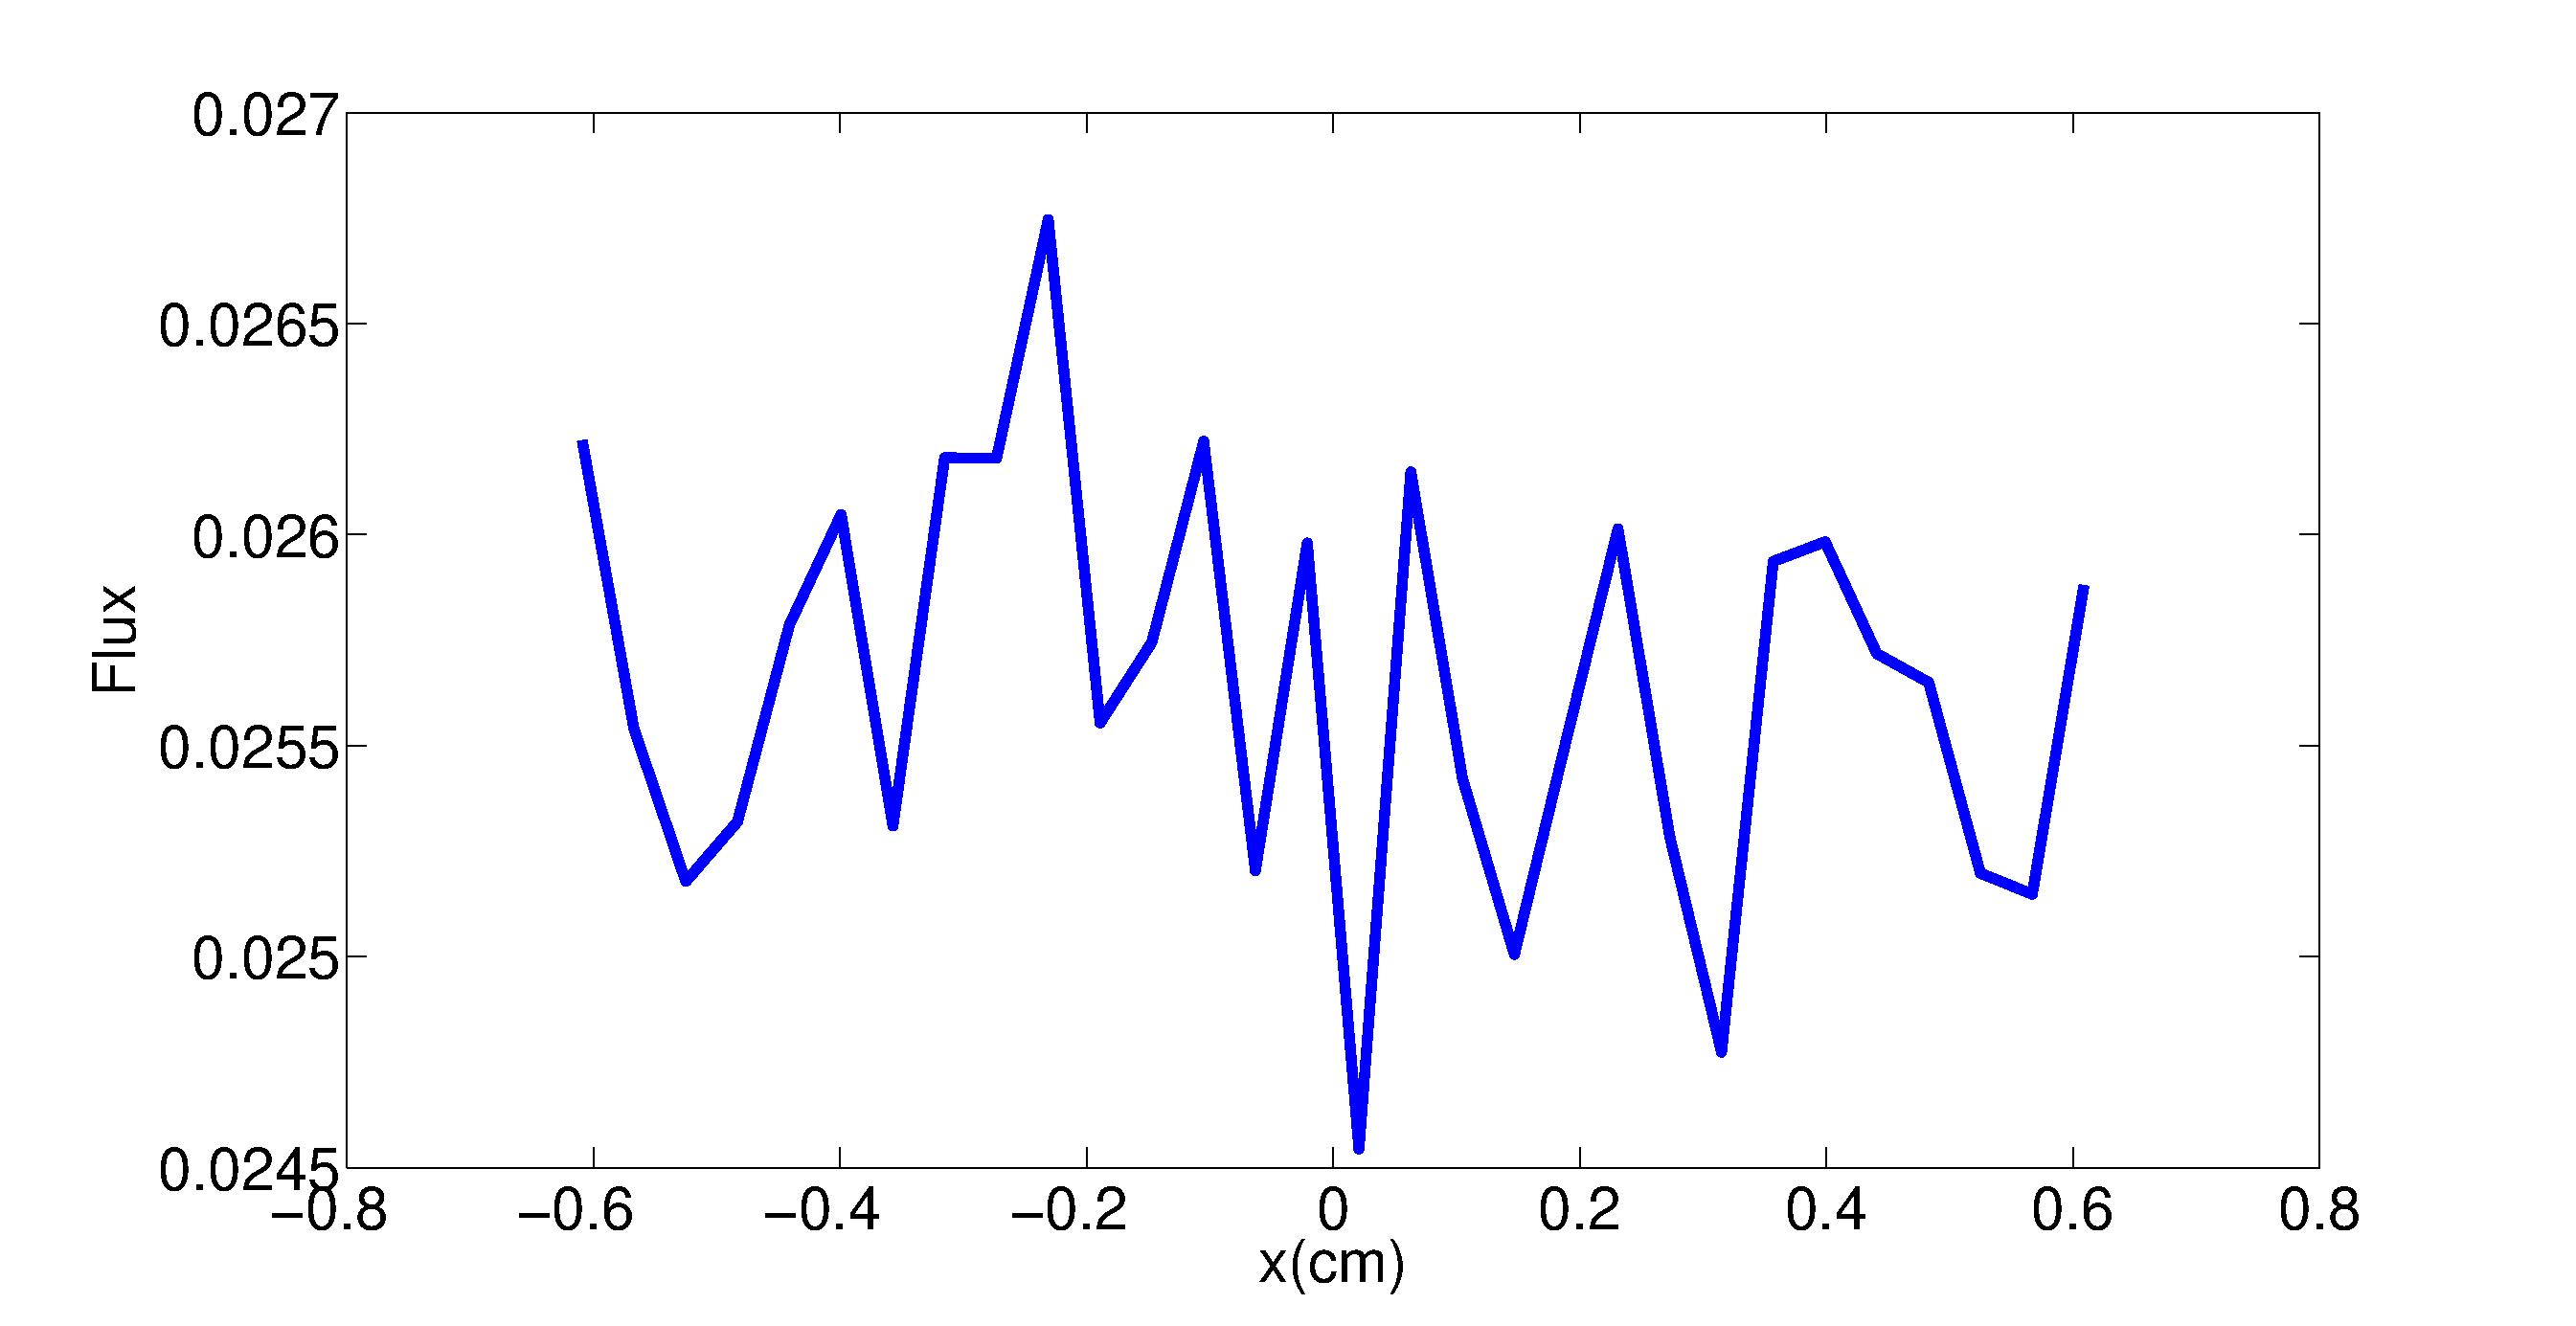
\includegraphics[width = \textwidth]{prob5_x.eps}
\end{figure}

\end{document}